\RequirePackage[T1]{fontenc}
\documentclass[conference,letterpaper]{IEEEtran}
\usepackage{cite}
\usepackage{amsmath,amssymb}
\interdisplaylinepenalty=2500
\usepackage{graphicx}
\usepackage{array}
\usepackage{booktabs}
\usepackage{url}
\graphicspath{{./figures/}}
\setlength{\textfloatsep}{12pt plus 2pt minus 2pt}
\setlength{\dbltextfloatsep}{12pt plus 2pt minus 2pt}
\hyphenation{op-tical net-works semi-conduc-tor}
\begin{document}


\title{Real-Time Cyber Attack Detection Using IoT-Based Electric Measurement Units at the Point of Common Coupling (PCC)}
\author{\IEEEauthorblockN{Abolfazl Najar, Thomas Prybylski, He Yang, Jin Ye, and WenZhan Song}
\IEEEauthorblockA{\textit{College of Engineering, University of Georgia}\\
Athens, Georgia, USA\\
\{Najar, Thomas.Prybylski, HeYang95, Jin.Ye, wsong\}@uga.edu}}
\maketitle
\raggedbottom

\begin{abstract}
False data injection attacks (FDIAs) on motor-current feedback can disturb grid-edge loads while remaining difficult to identify from aggregate measurements. A low-cost detection framework is developed using an IoT-enabled electric measurement unit (EMU) at the point of common coupling (PCC). Plug-and-play EMUs can be deployed in large numbers, with voltage/current feature reporting supported up to 60~Hz. A two-motor testbed is operated at different speeds and loads, and phase-current feedback biases are injected into either an AC induction motor or a permanent-magnet synchronous motor while both motors operate. PCC features are processed by a multihead convolutional neural network and bidirectional gated recurrent unit (CNN--Bi-GRU), with raw and temporal-difference inputs and rebalanced task losses. An accuracy of 93.46\% and attack recall of 95.32\% are obtained; the attacked motor is identified correctly in every attack window when evaluated conditional on attack. Real-time window processing is supported by a mean CPU processing time of 4.50~ms. The results demonstrate FDIA detection and source identification from aggregate PCC measurements, supporting wider grid-edge monitoring with lower-cost instrumentation.
\end{abstract}

\section{Introduction}
Power distribution has been transformed by Internet of Things (IoT) connectivity, with advanced monitoring enabled at the consumer edge. The attack surface has also been expanded: False Data Injection Attacks (FDIAs)~\cite{liu2009} can be applied as analog-to-digital converter (ADC) offsets on phase-current feedback, and communications can be disrupted. Subtle temporal deviations must therefore be identified from electrical measurements.

High-fidelity monitoring is provided by Phasor Measurement Units (PMUs) and micro-PMUs, but hardware and deployment requirements are increased by high reporting rates and Global Positioning System (GPS) synchronization~\cite{vonmeier2017}. Widespread consumer-edge visibility is consequently constrained by instrumentation cost.

To address this critical visibility gap, low-cost Electric Measurement Units (EMUs) are deployed at the PCC of a cyber-physical motor-drive testbed. Alternating-current (AC) features are acquired using an embedded ADE metering chip and an ESP32 microcontroller, then transmitted through built-in IoT connectivity for real-time edge window processing. The hardware platform is described in a companion manuscript submitted for publication~\cite{najarEMU2026}; related smart-plug PCC measurements have also been used for battery state-of-charge estimation~\cite{najarSOC2026}. EMU hardware requires only a small share of micro-PMU instrumentation cost, and plug-in installation is intended to reduce deployment overhead for widespread monitoring~\cite{najarEMU2026,vonmeier2017}.

An Intrusion Detection and Mitigation System (IDMS) using Deep Learning Neural Networks (DLNNs) and Long Short-Term Memory (LSTM) networks was proposed for FDIAs targeting Intelligent Electronic Devices (IEDs)~\cite{aljohani2024}. Its digitalized-substation sensing setup differs from the motor-drive PCC setting studied here, so its reported performance provides context rather than a direct benchmark.

An LSTM-based Variational Autoencoder (VAE) was developed for anomaly detection in unsupervised power-grid data~\cite{guha}. Similarly, anomaly detection using PMU streams has been investigated through comparative evaluations of machine learning models~\cite{pmu_lstm_2025}. Different datasets and sensing arrangements were used in these studies. A contextual comparison is provided in Table~\ref{tab:prior_work}; the published accuracies are not treated as directly comparable benchmarks.

\begin{table}[!t]
\centering
\caption{Comparison with existing electrical anomaly-detection and PCC-monitoring methods. Different datasets and sensing setups were used; the comparison concerns task and sensing scope.}
\label{tab:prior_work}
\small
\setlength{\tabcolsep}{3pt}
\begin{tabular}{@{}p{.28\linewidth}p{.30\linewidth}p{.35\linewidth}@{}}
\toprule
Work & Sensing/setting & Objective \\
\midrule
Aljohani et al.~\cite{aljohani2024} & IED/substation & FDIA detection and mitigation \\
Guha et al.~\cite{guha} & Grid phasor time series & Unsupervised anomaly detection \\
Dasari et al.~\cite{pmu_lstm_2025} & PMU/IEEE 39-bus & Multiclass anomaly detection \\
Najar et al.~\cite{najarSOC2026} & Smart-plug PCC & Battery state-of-charge estimation \\
Proposed & EMU/two-motor PCC & FDIA detection, motor and phase identification \\
\bottomrule
\end{tabular}
\end{table}


An EMU-based PCC solution is motivated by the instrumentation requirements of PMU/IED-centric methods. The key contributions are:
\begin{itemize}
    \item \textbf{Low-cost EMU-based PCC cyber-attack detection:} Real-time FDIA detection using IoT-enabled EMU measurements at the PCC of the tested two-motor system.
    \item \textbf{Hybrid deep model + training pipeline for imbalanced time-series:} Raw and temporal-difference features are combined with rebalanced multihead training for detection and identification.
    \item \textbf{Motor identification and operating-condition coverage:} Source identification while both motors operate, including 596 shared configurations and 12 recorded motor--speed--load combinations.
\end{itemize}

\section{Testbed Design and Dataset Structure}

\subsection{Testbed Design and Cyber-Attack Generation}
The experimental platform is illustrated in Figs.~\ref{fig:power_flow} and~\ref{fig:testbed_photo}. An AC induction motor (ACIM) and a permanent-magnet synchronous motor (PMSM) are operated simultaneously. An EMU is connected at their common PCC, where their aggregate electrical behavior is measured. One motor is attacked at a time; only PCC features are supplied to the classifier.
While PCC sensing is the focus of this study, stator current and voltage data at the motor-level are also available in the dataset for auxiliary monitoring and validation, and can be shared upon request for interested researchers.

\begin{figure}[!t]
    \centering
    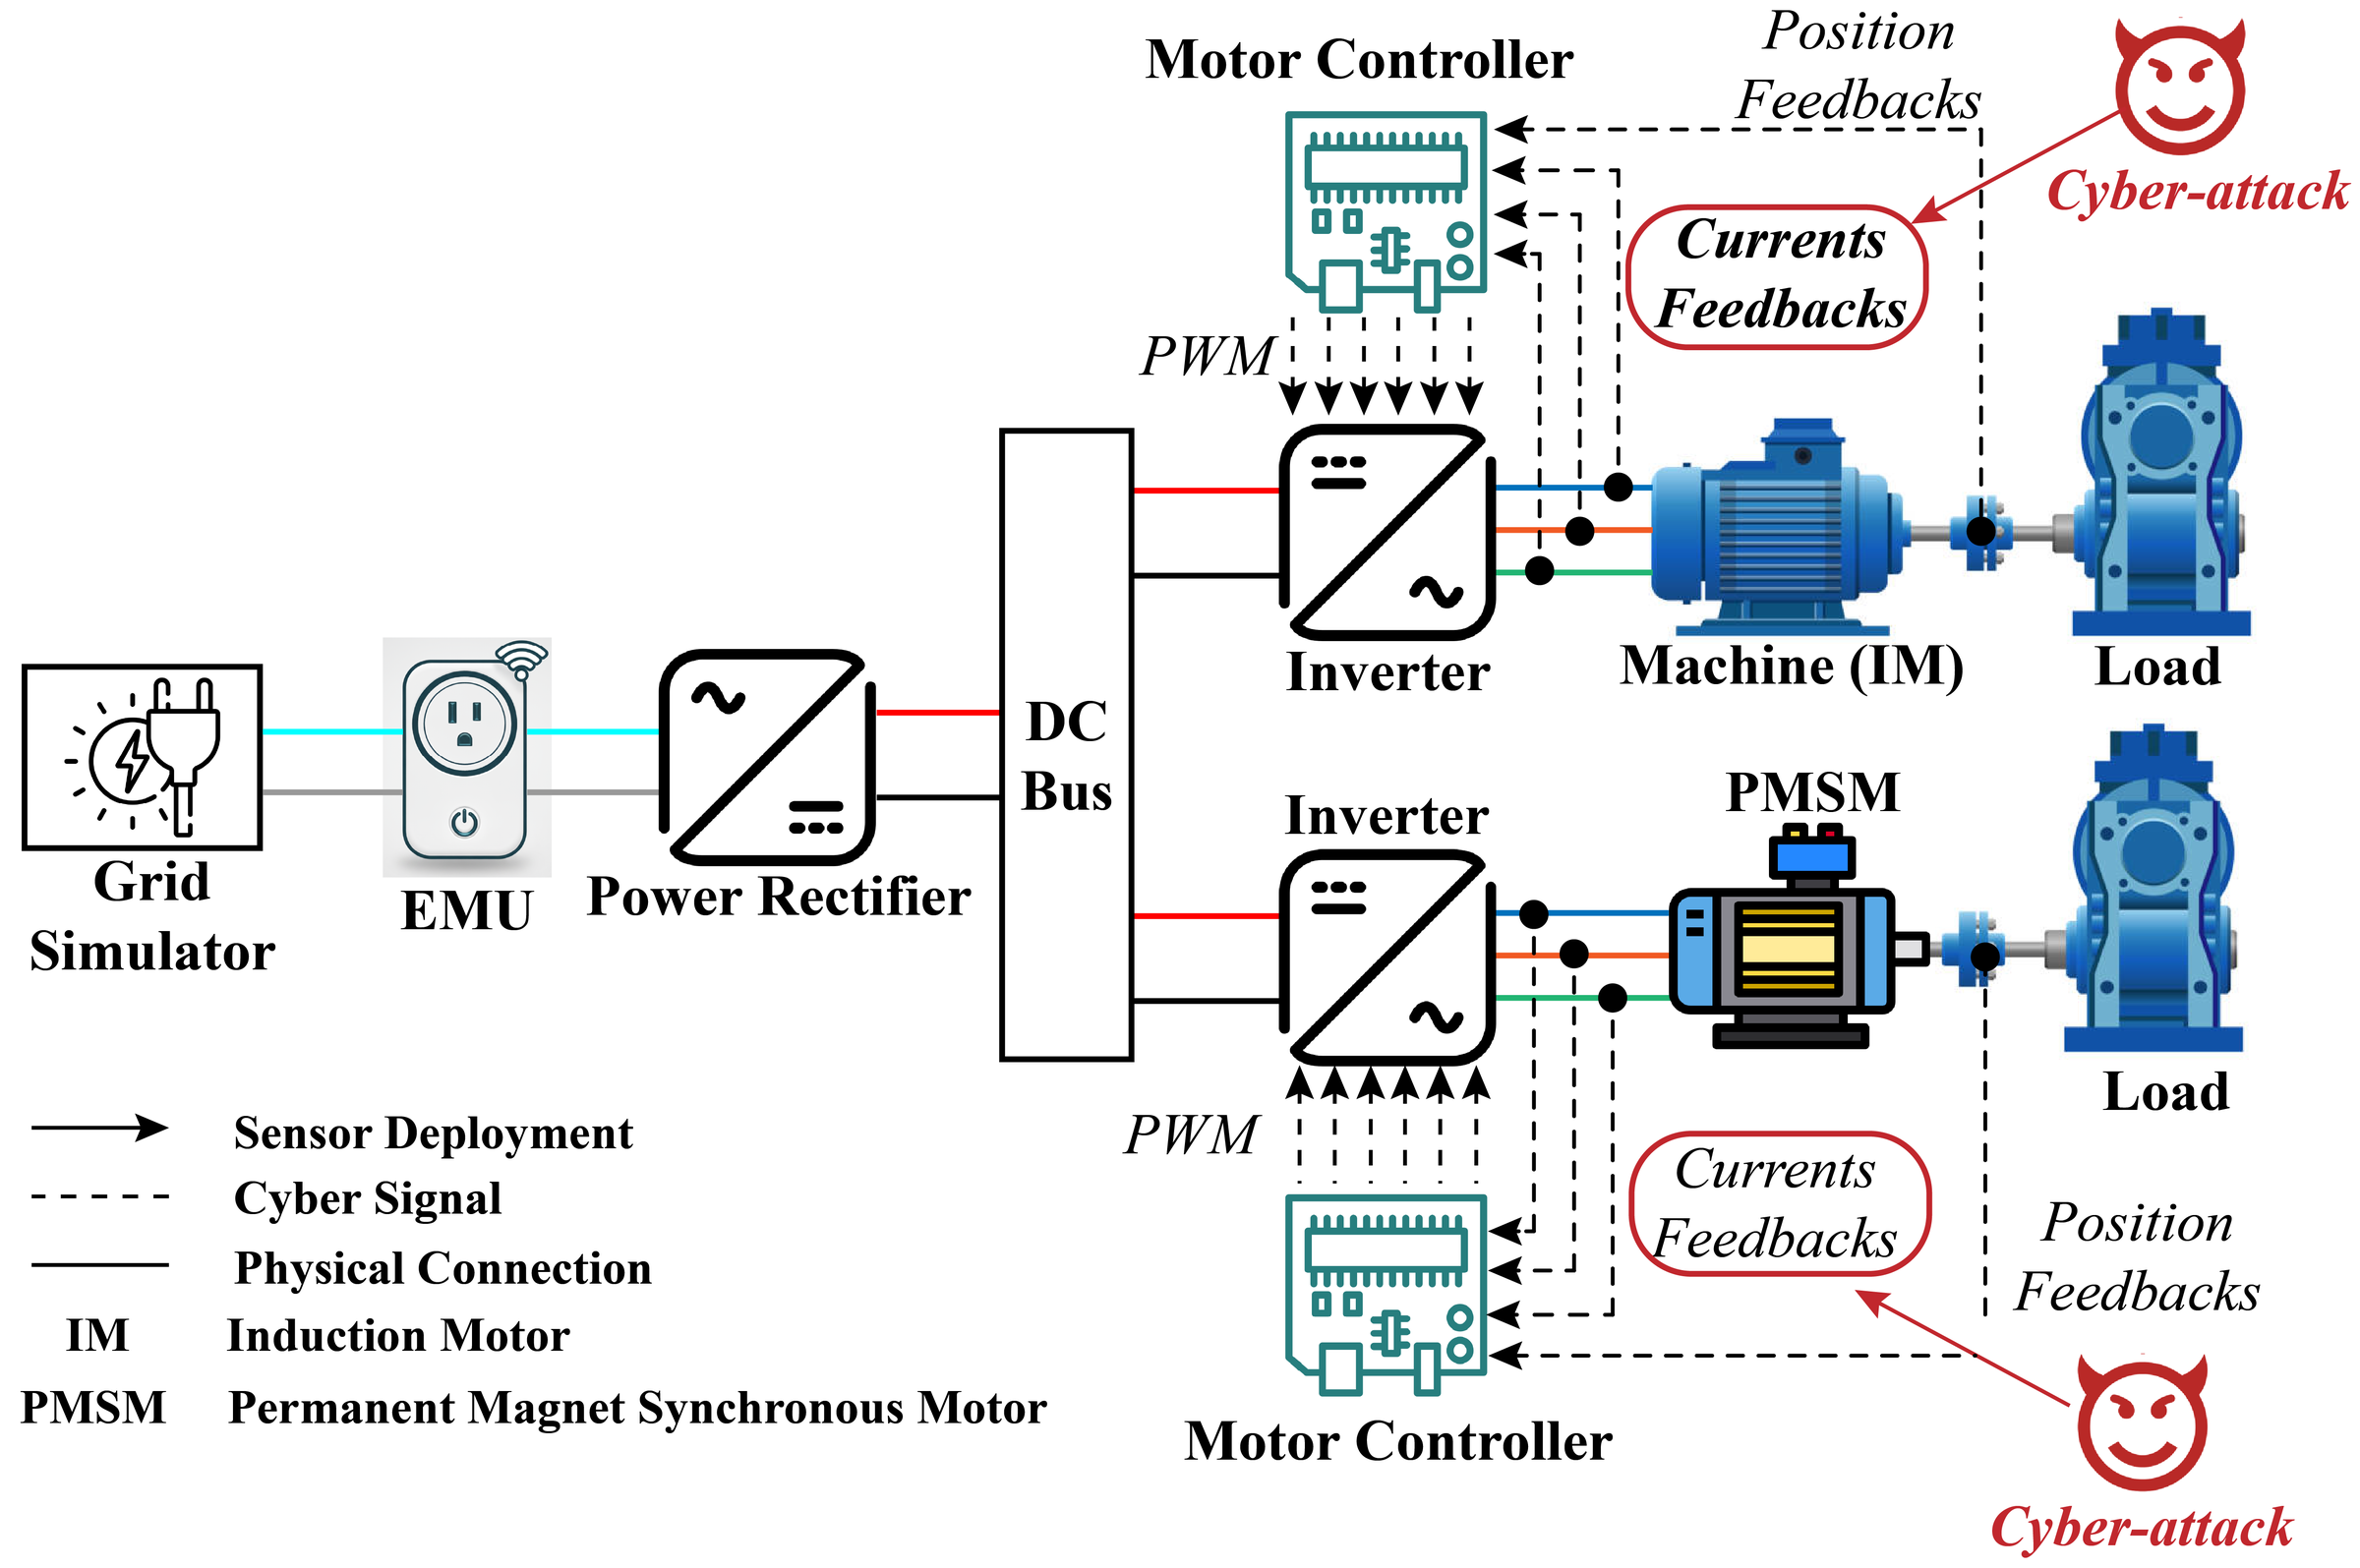
\includegraphics[width=\linewidth]{figures/power_flow_apec2027.png}
    \caption{Schematic diagram of designed multi-motor testbed for applying FDIA}
    \label{fig:power_flow}
\end{figure}
\begin{figure}[!t]
    \centering
    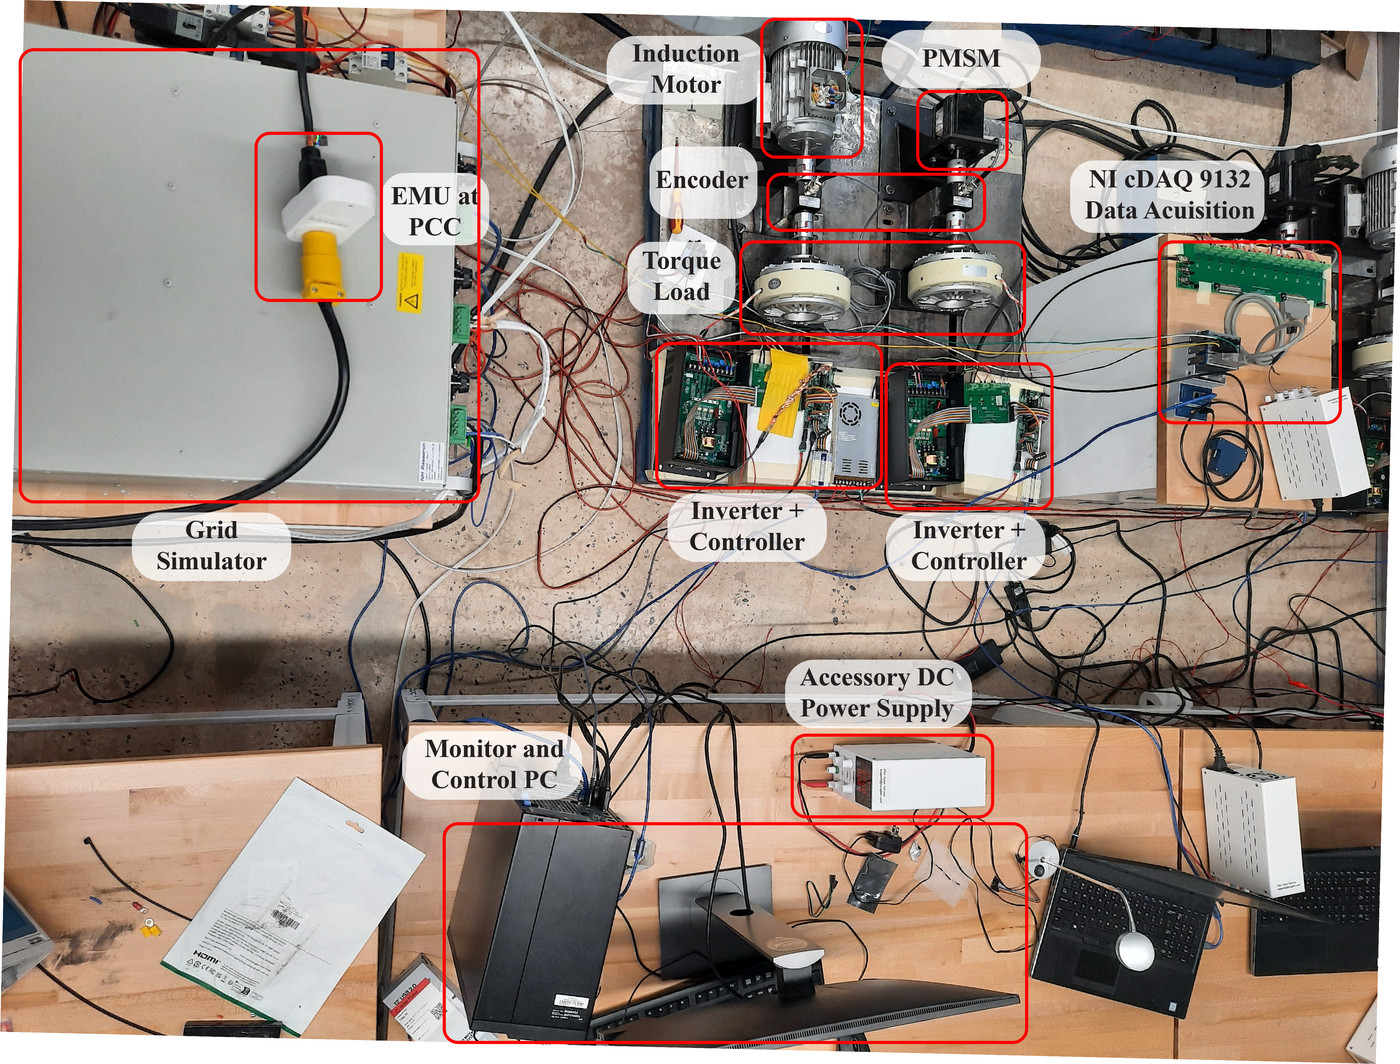
\includegraphics[width=\linewidth]{figures/testbed_apec2027.jpg}
    \caption{Physical Implementation of Schematic diagram of designed multi-motor testbed}
    \label{fig:testbed_photo}
\end{figure}
To safely emulate cyber incidents, false data injection attacks (FDIAs) are executed through pre-embedded firmware routines that introduce an offset-style bias injection on phase-current feedback signals. The attack model is defined as:
\begin{equation}
\tilde{\mathbf{i}}_{abc}(t) = \mathbf{i}_{abc}(t) + \boldsymbol{\alpha},
\end{equation}
where $\mathbf{i}_{abc}(t)$ is the true three-phase current vector and $\boldsymbol{\alpha}$ is the injected per-unit bias (applied per phase). Trials vary operating conditions (speed and load) and injection configurations (single-phase, two-phase, and multi-point), with attack magnitudes swept over $\alpha \in \{0.00025,\ldots,0.00500\}$ pu. Each run includes steady-state operation, attack activation, and recovery, enabling scalable supervised labeling.

\subsection{Dataset Structure}
The continuous PCC time-series is segmented using an overlapping sliding window with length 128 time steps and stride 16. Each sample is represented as $X \in \mathbb{R}^{128 \times 16}$, where the 16 EMU features summarize voltage and current measurements (e.g., amplitude, phase, root mean square (RMS), and total harmonic distortion (THD)).

This structure supports real-time binary detection and condition-aware studies such as motor, phase, severity and onset tasks. The 13 metadata fields are summarized in Table~\ref{tab:dataset_schema}. The binary label is 1 if any sample in the window is attacked. Attack and phase flags are max-pooled; the first attack index is stored as the onset label. Normal phase labels are $(A,B,C)=(0,0,0)$, and ROCOF denotes rate of change of frequency. Stored severity labels are evaluated separately from the physical injection parameter $\alpha$.

Normal and attack feature windows are compared in Fig.~\ref{fig:signal_windows}; phase, frequency, and THD time-series examples are provided in Fig.~\ref{fig:feature_timeseries}.
\begin{figure}[!t]
    \centering
    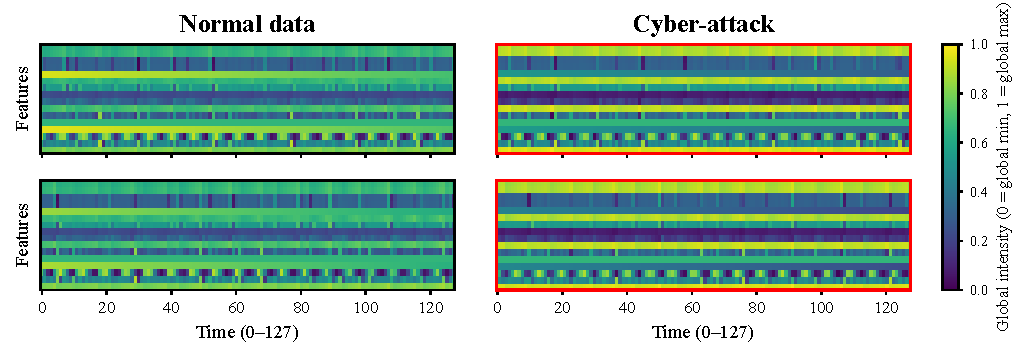
\includegraphics[width=\linewidth]{figures/signals_apec2027.pdf}
    \caption{Normal vs Cyber-attack data}
    \label{fig:signal_windows}
\end{figure}
\begin{table*}[!t]
\centering
\caption{Dataset Input ($X$) and Label ($y$) Schema}
\label{tab:dataset_schema}
\begin{tabular}{l|l|c}
\hline
\textbf{Input (X)} & \textbf{Features} & \textbf{Count} \\ \hline
Current Features & Amp, Amp$_2^*$, Freq, Freq$_2^*$, Phase, RMS, ROCOF, THD & 8 \\
Voltage Features & Amp, Amp$_2$, Freq, Freq$_2$, Phase, RMS, ROCOF, THD & 8 \\ \hline
\textbf{Output (y)} & \textbf{Description} & \textbf{Scope} \\
\hline
\texttt{is\_attack} & Binary (0=Normal, 1=Attack) & 2 \\
\texttt{is\_onset} & First attack index (0--127); $-1$ if absent & $128+1$ \\
\texttt{attack\_type} & Attack mode (normal:0, cyber\_attack:1) & 2 \\
\texttt{Motor} & 0=None, 1=ACIM, 2=PMSM & 3 \\
\texttt{A, B, C} & Phase-specific injection flags (0 and 1) & 2 \\
$\text{sev}_A, \text{sev}_B, \text{sev}_C$ & Stored severity per phase (0.025, 0.050, \ldots, 0.500) & 20 \\
\texttt{speed} & Motor speed settings (700, 1000, and 1300 RPM) & 3 \\
\texttt{load} & Motor torque load settings (2, 3, and 4) & 3 \\
\texttt{attack\_id} & Unique event identifier & 2727 \\ \hline
\multicolumn{3}{l}{$^*$Amp$_2$ and Freq$_2$ denote the second dominant amplitude and frequency components.} \\
\end{tabular}
\end{table*}
\begin{figure}[!t]
    \centering
    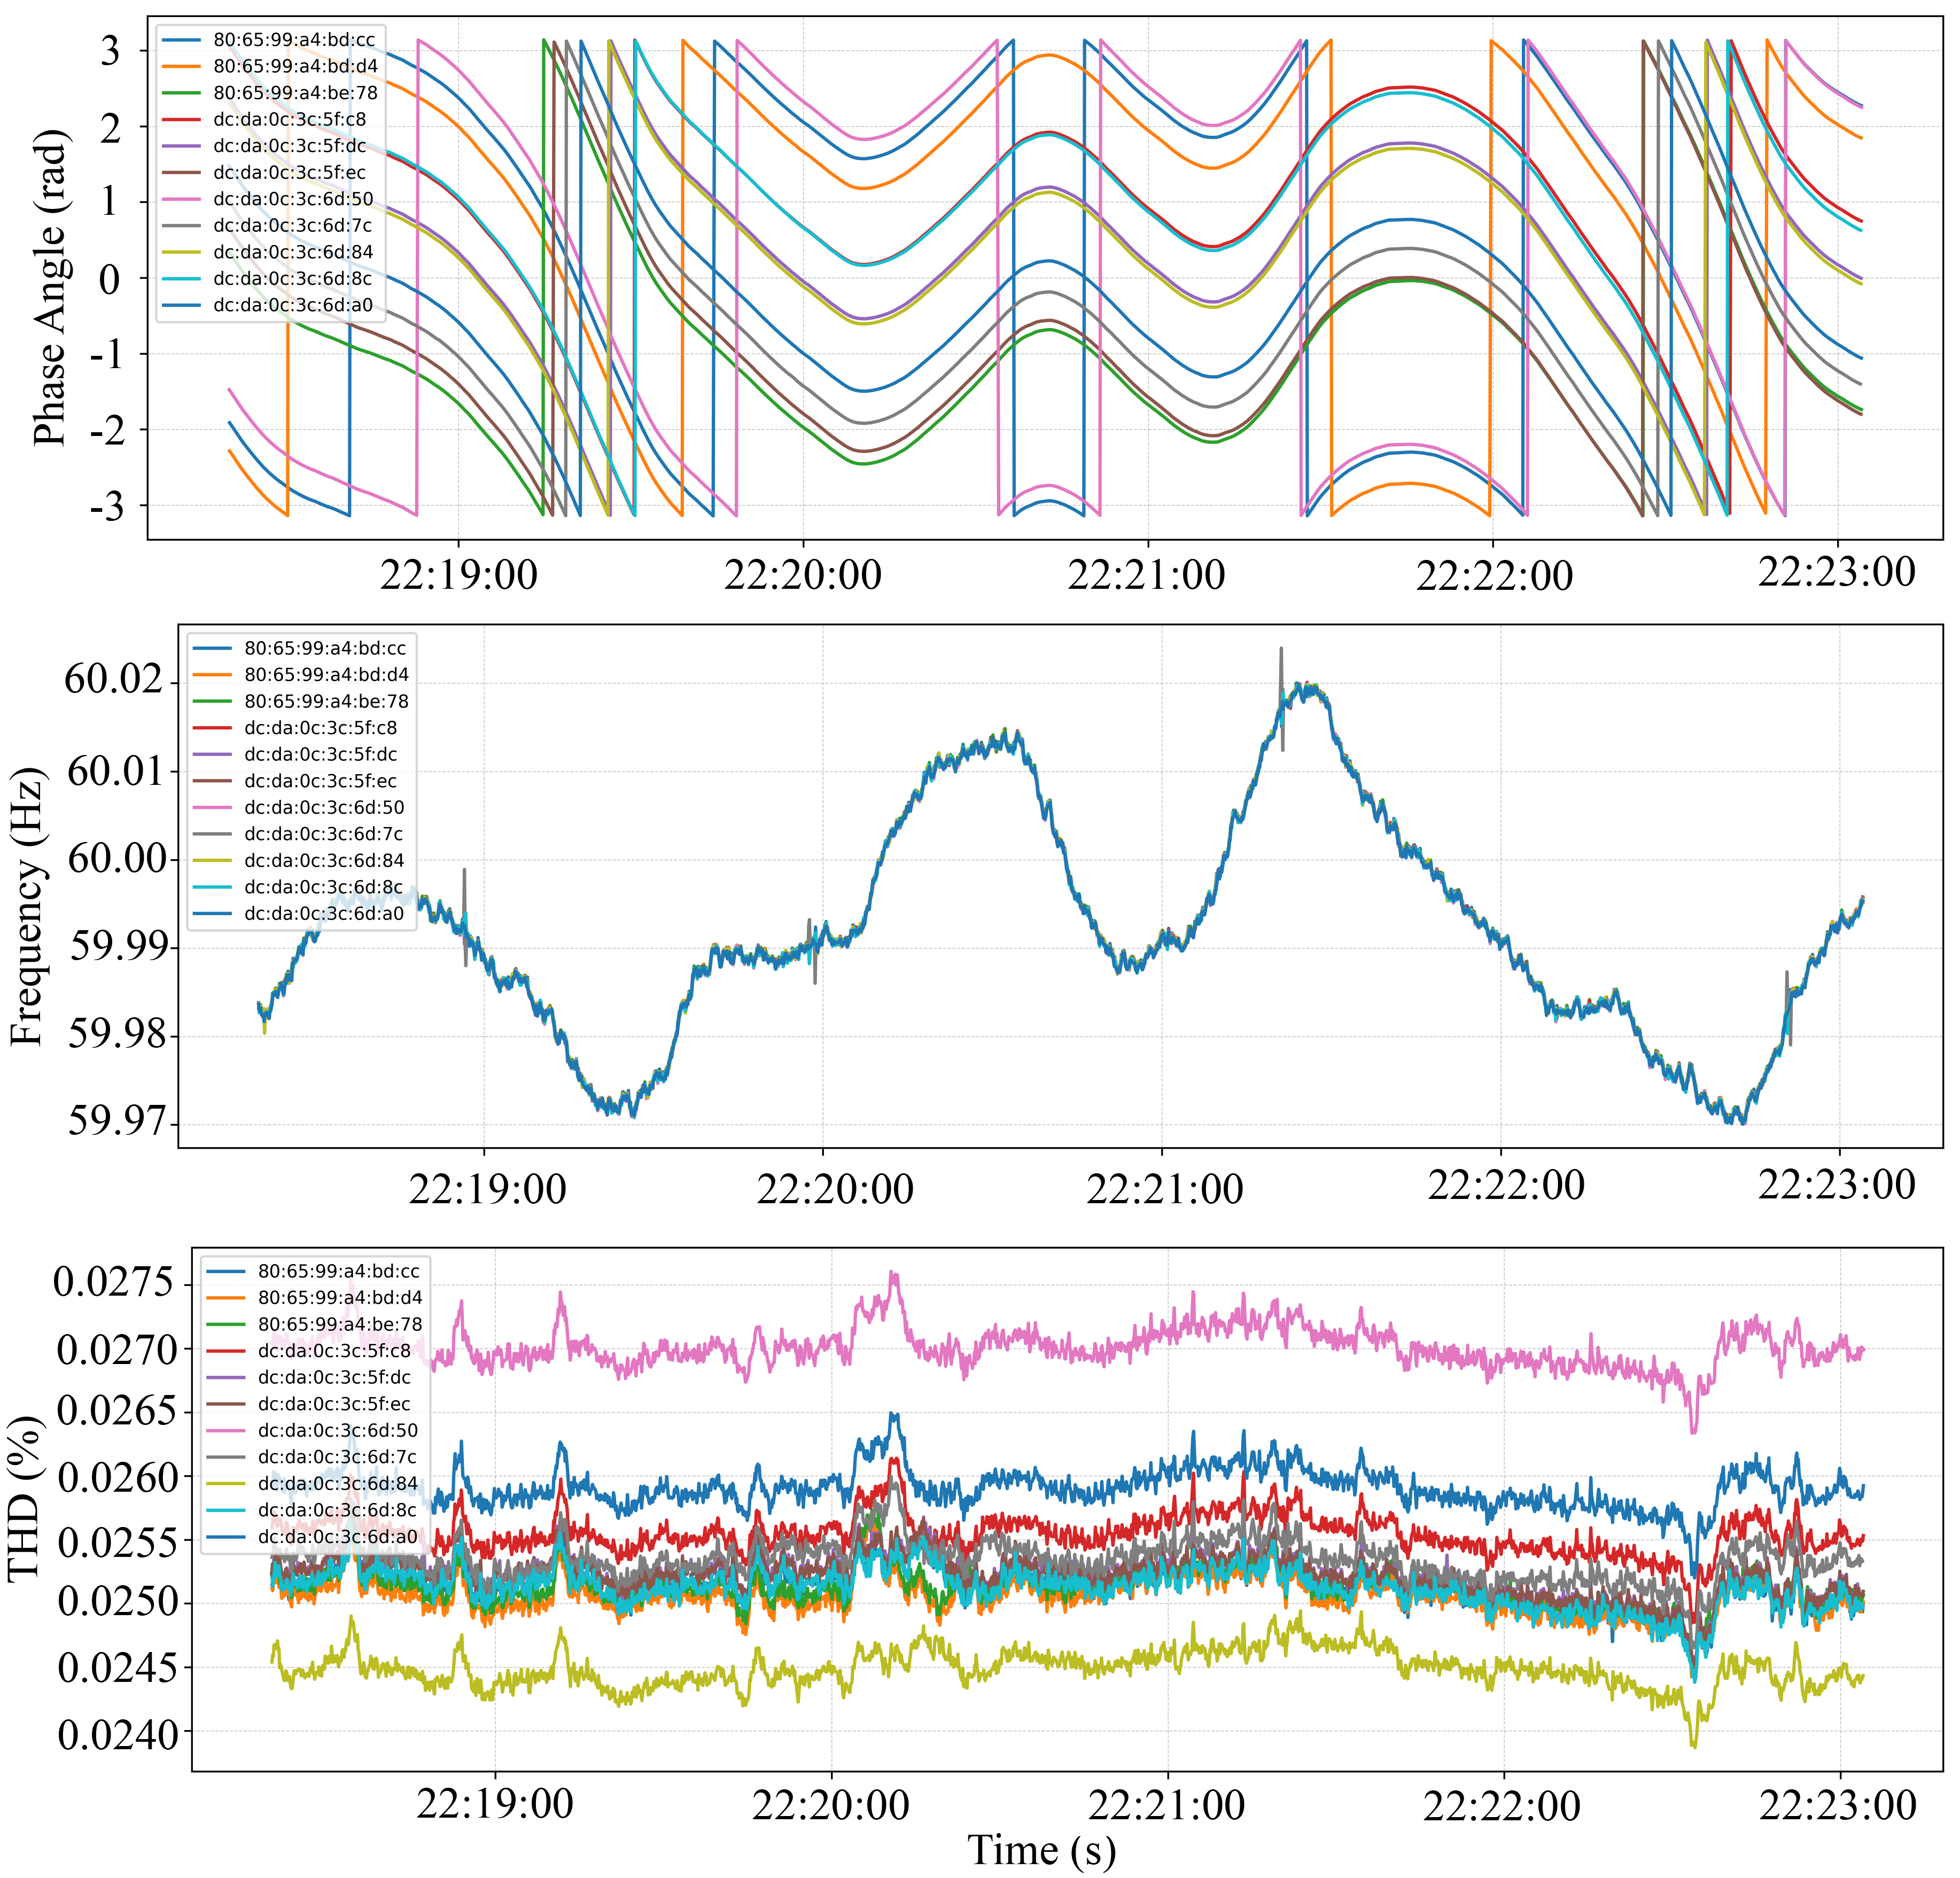
\includegraphics[width=\linewidth]{featurescombined.png}
    \caption{Comparative time-series visualization of EMU phase, frequency, and THD measurements.}
    \label{fig:feature_timeseries}
\end{figure}

\section{Bidirectional GRU Architecture}

A CNN--Bi-GRU network is used because subtle temporal deviations must be distinguished from isolated point events. Gated recurrence~\cite{cho2014} and bidirectional sequence processing~\cite{schuster1997} are combined within each completed observation window.

The preprocessing and shared six-head network are illustrated in Fig.~\ref{architecture}. Each $128\times16$ window is expanded to $128\times32$ by the temporal feature construction described below.
The classifier comprises two Conv1D blocks (64 filters, kernel size 3) with Batch Normalization, followed by a Bidirectional GRU for sequence modeling. Local temporal patterns are extracted by Conv1D filters across input channels. Retained state is controlled by GRU update/reset gates, and each completed window is processed forward and backward to combine context. Outputs are aggregated with GlobalAveragePooling1D, passed through a 64-unit dense layer with 30\% dropout, and mapped to six parallel heads: attack (one sigmoid), motor (two-class softmax), phases (three sigmoids), severity (three sigmoids), start presence (one sigmoid), and start position (one sigmoid). The shared Bi-GRU has 64 units per direction; the model has 77,963 parameters.
\begin{figure*}[t]
    \centering
    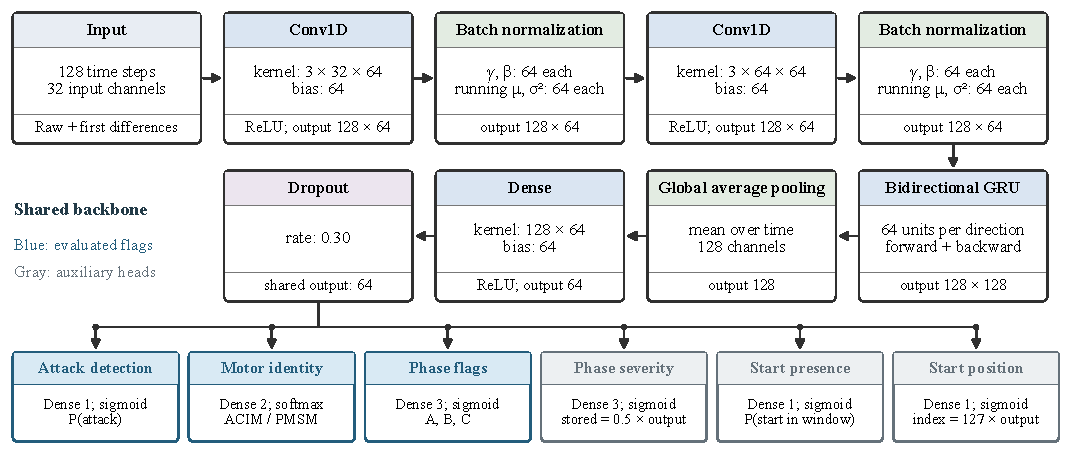
\includegraphics[width=\textwidth]{figures/architecture_rebalanced_apec2027.pdf}
    \caption{The evaluated multihead CNN--Bi-GRU. Six parallel output heads share the convolutional and recurrent representation. Blue heads provide attack, motor, and phase classifications; gray heads are auxiliary severity/timing outputs.}
    \label{architecture}
\end{figure*}


Regularization is provided by Batch Normalization, dropout, and early stopping. The reported fine-tuning run uses Adam at $3\times10^{-4}$, batch size 128, gradient-norm clipping at 1, and patience 12. The learning rate is halved after five unimproved epochs, with a minimum of $10^{-5}$.

\subsection{Addressing Class Imbalance}
Approximately 80\% of the windows are attack-labeled. All training windows are retained without under/oversampling. Rebalanced fine-tuning is performed with training-derived, fixed inverse-frequency attack weights: 2.5445 for normal and 0.6223 for attack. Motor identity is trained using standard two-class categorical cross-entropy: a larger loss is assigned when the correct motor receives a smaller predicted probability. Only attack windows are included, with inverse-frequency motor-class weights. For each phase, half the loss weight is assigned to affected labels, with one quarter each assigned to normal zeros and unaffected phases during attacks.

\subsection{Temporal Feature Engineering}
First-order differences are computed with sequence length preserved by prepending the first time step, then concatenated with the raw features. The resulting representation is feature-wise standardized, providing both absolute-state context and rate-of-change dynamics.


\subsection{Multihead Loss and Evaluation Protocol}
The windows are partitioned 80/20 by stratified sampling at seed 42: 94,157 training and 23,540 evaluation windows (4,626 normal; 18,914 attack). The evaluation partition is used for checkpoint selection. Adjacent windows share 112 of 128 samples, and recordings can occur in both partitions.

A pretrained multihead checkpoint is fine-tuned for 45 epochs. The implemented objective is
\begin{equation}
 \mathcal{L}=\sum_{k\in\{a,m,p,s,o,t\}}\lambda_k\mathcal{L}_k,
 \qquad \lambda_k\equiv1,
 \label{eq:multitask_loss}
\end{equation}
where $a,m,p,s,o,t$ denote attack, motor, phases, severity, start presence, and start position. All six outer coefficients remain fixed; no adaptive task weighting is applied. Training-derived class weights and masks are retained within each loss, so equal coefficients do not imply equal gradient contributions.

Weighted binary cross-entropy is used for attack, phases, and start presence. Motor categorical cross-entropy is evaluated only on attack windows. For severity targets divided by 0.5, $\mathcal{L}_s=0.5\,\mathrm{MAE}_{+}+0.5\,\mathrm{MSE}_{+}+0.05\,\mathrm{MAE}_{-}$, where $+$/$-$ denote affected/unaffected phase labels. Position targets are divided by 127, and MAE is evaluated only for known starts.

Checkpoints are selected by the mean of six task utilities: attack balanced accuracy, conditional motor balanced accuracy, phase balanced accuracy averaged over all/attack windows, start-presence F1, and two regression utilities. Each regression utility is $\max(0,\min(1,1-E/(2E_{\rm ref})))$, using MAE $E$ and the error $E_{\rm ref}$ of a training-median reference. Epoch 45 is selected.

\section{Experimental Results}

Since cyber-attack detection prioritizes missed-attack reduction, performance is tracked using precision, recall, F1, balanced accuracy, and accuracy.

Attack and phase outputs use the fixed threshold 0.5. With rebalanced training, dual-stream (raw+differential) inputs, and the CNN--Bi-GRU architecture, an accuracy of 93.46\%, balanced accuracy of 90.59\%, precision of 96.50\%, and attack recall of 95.32\% are obtained. Normal-window false positives are 14.14\%; average precision is 0.9937 and ROC-AUC is 0.9758 (area under the receiver operating characteristic curve). Detection errors are shown in Fig.~\ref{fig:confusion_matrix}; attack recall across stored severity groups is shown in Fig.~\ref{fig:Severityeffect}.

The LSTM, CNN--LSTM, CNN--Bi-GRU, and proposed results are compared in Table~\ref{tab:comparison}. The three reference models were trained with identical inputs, partition, width 64, Adam learning rate $10^{-3}$, batch size 128, and attack-loss class weights 1.0/1.5 for at most 40 epochs. Checkpoints were selected by balanced accuracy at threshold 0.5. Additional multihead pretraining and rebalanced fine-tuning were applied to the proposed model; complete pipelines are compared, rather than isolated architecture effects.


\begin{table}[!t]
\centering
\caption{Binary FDIA detection performance. Rates are percentages; FPR denotes false-positive rate.}
\label{tab:comparison}
\setlength{\tabcolsep}{3pt}
\small
\begin{tabular}{lrrrr}
\toprule
Model & Accuracy & Bal. acc. & Recall & FPR \\
\midrule
LSTM & 84.89 & 64.15 & 98.33 & 70.04 \\
CNN--LSTM & 89.81 & 85.33 & 92.71 & 22.05 \\
CNN--Bi-GRU & 89.00 & 85.16 & 91.49 & 21.16 \\
\midrule
CNN--Bi-GRU (proposed) & 93.46 & 90.59 & 95.32 & 14.14 \\
\bottomrule
\end{tabular}
\end{table}





\begin{figure}
    \centering
    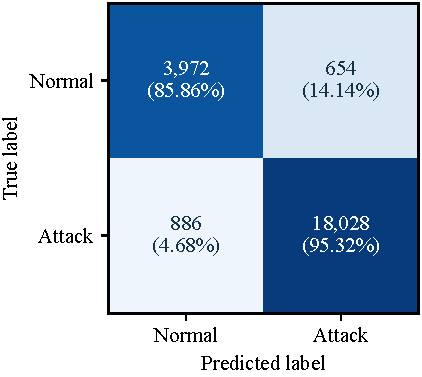
\includegraphics[width=\linewidth]{figures/confusion_matrix_rebalanced_author.pdf}
    \caption{Binary FDIA detection confusion matrix at threshold 0.5.}
    \label{fig:confusion_matrix}
\end{figure}

\begin{figure}[!t]\centering
    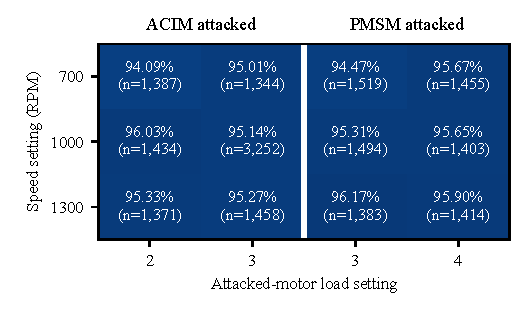
\includegraphics[width=\linewidth]{figures/operating_conditions_rebalanced.pdf}
    \caption{Attack recall and attack-window counts for all 12 recorded operating conditions. Both motors operate; labels identify the attacked motor's settings. Threshold 0.5 is fixed throughout.}
    \label{fig:operating_conditions}
\end{figure}

\begin{figure*}[!t]
    \centering
    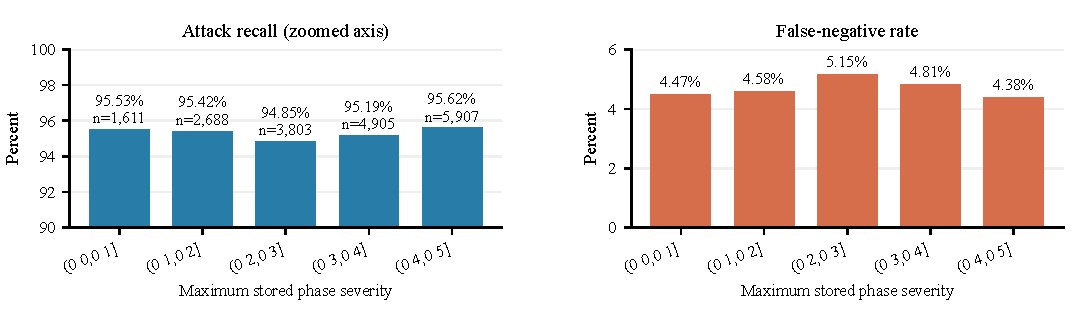
\includegraphics[width=\textwidth]{figures/severity_group_recall_rebalanced.pdf}
    \caption{Attack recall and false-negative rate in stored severity groups, from the selected rebalanced model.}
    \label{fig:Severityeffect}
\end{figure*}



\begin{figure*}[!t]\centering
    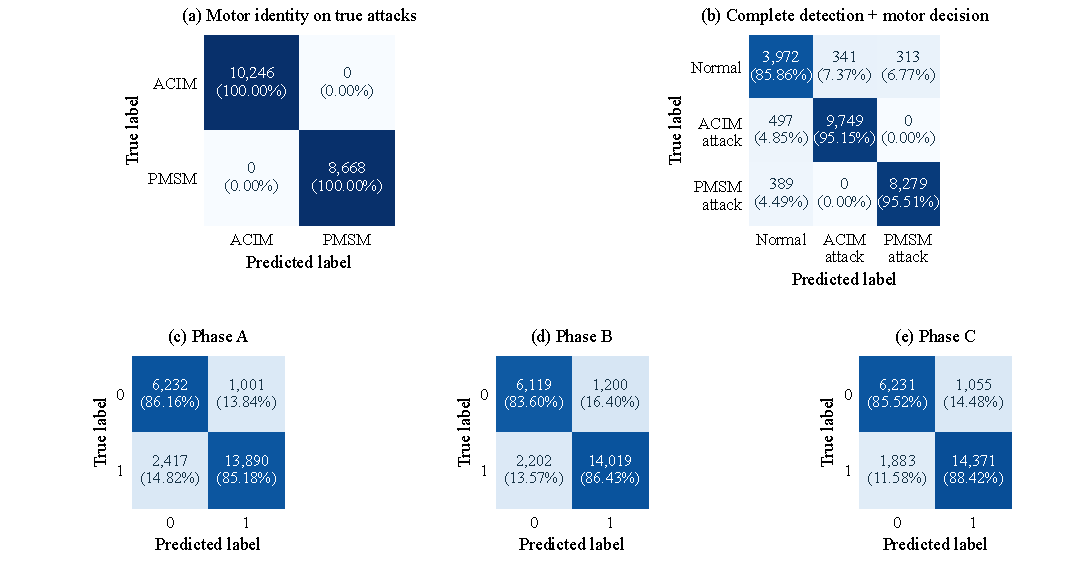
\includegraphics[width=\textwidth]{figures/classification_confusion_rebalanced.pdf}
    \caption{Motor identity conditional on true attacks, complete detection-plus-motor decisions, and raw phase A/B/C confusion matrices. Normal zero-phase labels are included in phase evaluation. Cells show counts and true-row percentages; phase 0/1 denotes unaffected/attacked.}
    \label{fig:joint_outputs}
\end{figure*}

\subsection{Real-Time Processing Feasibility}
For the approximately 7-Hz recordings used here, an 18.29-s nominal window and 2.29-s update interval are obtained from 128 samples and stride 16. The up-to-60-Hz device capability is separate from this recording rate. Processing 1,000 validation windows (batch 1, 50 warm-ups) on an Intel Core Ultra 9 285K CPU with four threads (TensorFlow 2.21) is completed in 4.50~ms mean, 5.19~ms 95th-percentile, and 9.26~ms maximum, including preprocessing, all six heads, and decoding. The update interval is met in every measured call, supporting real-time window processing on this host. Window duration is not attack-to-alarm delay; acquisition, communication, and event-detection delays remain unmeasured.


\subsection{Motor and Phase Identification}
All 10,246 ACIM and 8,668 PMSM attack windows are correctly identified by the motor head when evaluated conditional on true attacks. Including detector misses, correct detection plus identity is 95.32\%, and the complete normal/ACIM/PMSM decision has 93.46\% accuracy (Fig.~\ref{fig:joint_outputs}). This conditional 100\% identity result is distinct from complete-pipeline performance.

Raw phase outputs include all 23,540 windows, including normal $(0,0,0)$ labels. Exact ABC accuracy is 75.27\%, mean phase balanced accuracy is 85.88\%, and macro-F1 is 0.8965. Predicting 111 for every window gives 57.85\% exact accuracy. On normal windows, 86.10\% have all flags correctly zero. The auxiliary severity MAE is 0.1243 on affected phases, versus 0.1226 for the training-median baseline; start-presence F1 is 0.425 and known-start position MAE is 19.23 samples. These auxiliary results do not support reliable severity/timing claims.





\subsection{Motor Identification under Common Configurations}
All 18,914 attack windows are used for the overall motor result in Table~\ref{tab:matched_motor_settings}. An additional control is provided by selecting only speed, load, phase-flag, and stored phase-severity tuples represented for both attacked motors. Of the attack windows, 8,841 satisfy this matching rule, spanning 596 shared tuples; the remaining 10,073 are retained in the overall result but excluded from this subset. Thus, 8,841 is a controlled subset, not the total attack cohort.

\begin{table}[!t]
\centering
\caption{Motor identification for 596 configurations represented for both attacked motors. All 8,841 windows are attack-labeled.}
\label{tab:matched_motor_settings}
\small
\setlength{\tabcolsep}{4pt}
\begin{tabular}{lrrr}
\toprule
\shortstack{Attacked\\motor} & \shortstack{Attack\\windows} & \shortstack{Conditional\\identity (\%)} & \shortstack{Detection +\\identity (\%)} \\
\midrule
ACIM & 4,475 & 100.00 & 95.26 \\
PMSM & 4,366 & 100.00 & 95.30 \\
Combined & 8,841 & 100.00 & 95.28 \\
\bottomrule
\end{tabular}
\end{table}


For the shared settings, conditional identity is 100\% and detection plus identity is 95.28\%. Identification from aggregate PCC features is therefore supported even when the recorded settings match between motor classes. Joint errors are caused by detector misses. The original evaluation windows are reused; no additional recording holdout is introduced.

\subsection{Coverage of Recorded Operating Conditions}
Across all 12 recorded motor--speed--load combinations, recall ranges from 94.09\% (ACIM, 700 RPM, load setting 2) to 96.17\% (PMSM, 1300 RPM, load setting 3), at the same threshold 0.5 (Fig.~\ref{fig:operating_conditions}). This supports consistent attack sensitivity across represented settings.



\section{Conclusion and Future Work}

FDIA detection and attacked-motor identification have been demonstrated from aggregate PCC measurements while both motors operate. Identification is supported across matching recorded settings, and consistent sensitivity is obtained across the represented speeds and loads. The fixed-weight multihead CNN--Bi-GRU can be processed within the measurement-update interval on the benchmarked CPU. The framework will be extended to benign transients and other faults, with additional motor counts and independent recordings evaluated before broader deployment.

Results use overlapping-window validation, with no independent recording test. Performance with ten motors remains unestablished and requires dedicated validation.

\section*{Acknowledgment}
OpenAI Codex assisted with manuscript revisions, evaluation code, and diagnostic figures. Reported metrics were computed from the recorded dataset.

\bibliographystyle{IEEEtran}
\bibliography{References_main}

\end{document}
